\documentclass[mathserif, handout]{beamer}

\usepackage{url}
% ======================================================================
% General LaTeX Setup for Beamer (Reusable Preamble)
% Author: Chandra Gummaluru
% ======================================================================

\documentclass[mathserif, handout]{beamer}
\setbeamertemplate{frametitle}{}

% ------------------------------------------------------------
% basic packages
% ------------------------------------------------------------
\usepackage{url}
\usepackage{ifthen}
\usepackage{enumerate}
\usepackage[font=small]{caption}
\usepackage{subcaption}
\usepackage{moresize}
\usepackage[outline]{contour}
\usepackage{transparent}
\usepackage{worldflags}
\usepackage{bm}
\usepackage{graphbox}
\usepackage{mathtools}
\usepackage{multirow}
\usepackage{fontawesome5}
\usepackage{pifont}
\usepackage{array}
\usepackage{comment}

% ------------------------------------------------------------
% math
% ------------------------------------------------------------
\DeclarePairedDelimiter{\floor}{\lfloor}{\rfloor}
\DeclarePairedDelimiter{\ceil}{\lceil}{\rceil}

% ------------------------------------------------------------
% colors
% ------------------------------------------------------------
\definecolor{hl}{RGB}{248,196,69}
\definecolor{myred}{HTML}{ED5565}
\definecolor{myorange}{HTML}{FC6E51}
\definecolor{myyellow}{HTML}{FFCE54}
\definecolor{mycyan}{HTML}{4FC1E9}
\definecolor{myblue}{HTML}{5D9CEC}

\newcommand{\graytext}[1]{\footnotesize\color{gray}#1\normalsize\color{black}}

% ------------------------------------------------------------
% symbols
% ------------------------------------------------------------
\newcommand{\cmark}{\ding{51}}
\newcommand{\xmark}{\ding{55}}

% ------------------------------------------------------------
% highlighting
% ------------------------------------------------------------
\newcommand{\reducedstrut}{\vrule width 0pt height .9\ht\strutbox depth .9\dp\strutbox\relax}
\newcommand{\highlight}[1]{%
  \begingroup\setlength{\fboxsep}{0pt}\colorbox{hl}{\reducedstrut$\displaystyle #1$\/}\endgroup}
\newcommand{\highlightc}[2]{%
  \begingroup\setlength{\fboxsep}{0pt}\colorbox{#1}{\reducedstrut$\displaystyle #2$\/}\endgroup}

% ------------------------------------------------------------
% environments (boxes)
% ------------------------------------------------------------
\usepackage{tcolorbox}
\tcbuselibrary{skins}

\newtcolorbox{thmbox}[1][]{colback=gray!30!white!20, colframe=black, fonttitle=\bfseries, title=#1, boxrule=0.5pt}

% 1) Bottom open (draw top + sides only)
\newtcolorbox{thmboxtop}[1][]{
    enhanced,
    frame hidden,
    colback=gray!30!white!20,
    borderline north={0.5pt}{0pt}{black}, % top
    borderline west={0.5pt}{0pt}{black},  % left
    borderline east={0.5pt}{0pt}{black}   % right
}

% 2) Top open (draw bottom + sides only)
\newtcolorbox{thmboxbot}[1][]{
    enhanced,
    frame hidden,
    colback=gray!30!white!20,
    borderline south={0.5pt}{0pt}{black}, % bottom
    borderline west={0.5pt}{0pt}{black},  % left
    borderline east={0.5pt}{0pt}{black}   % right
}

% 3) Side only (draw only left and right)
\newtcolorbox{thmboxside}[1][]{
    enhanced,
    frame hidden,
    colback=gray!30!white!20,
    borderline west={0.5pt}{0pt}{black},  % left
    borderline east={0.5pt}{0pt}{black}   % right
}

\newtcolorbox{defboxtop}[1][]{
    enhanced,
    colback=gray!30!white!20,
    frame hidden,
    overlay={
        % Draw top + sides with rounded corners
        \draw[line width=0.5pt, black, rounded corners=3mm]
            (frame.south west) -- (frame.north west) -- (frame.north east) -- (frame.south east);
    },
    #1
}

\newtcolorbox{defboxbot}[1][]{
    enhanced,
    colback=gray!30!white!20,
    frame hidden,
    overlay={
        % Draw top + sides with rounded corners
        \draw[line width=0.5pt, black, rounded corners=3mm]
            (frame.north west) -- (frame.south west) -- (frame.south east) -- (frame.north east);
    },
    #1
}

\newtcolorbox{defboxside}[1][]{
    enhanced,
    frame hidden,
    colback=gray!30!white!20,
    borderline west={0.5pt}{0pt}{black},  % left
    borderline east={0.5pt}{0pt}{black}   % right
}

\newtcolorbox{proofbox}[1][]{colback=gray!20!white!20, colframe=grey, fonttitle=\bfseries, title=#1, boxrule=0.5pt, colbacktitle=white, enhanced jigsaw, sharp corners}

% ------------------------------------------------------------
% code listings
% ------------------------------------------------------------
\usepackage{listings}
\lstdefinestyle{mypython}{
  language=Python,
  deletekeywords=[2]{open, next, from, chr, str, int},
  morekeywords=[3]{List, Graph, Tree, Dict, Set, UnionFind, Ordict, Trie, Queue},
  morekeywords=[4]{ListNode, Vertex, Edge, Path, TreeNode, DictNode, UnifNode, OrdictNode, TrieNode, QueueNode},
  morekeywords=[5]{True, False, Boolean, String, Integer, Key, Function, KeyedObject, Object, Array, Tuple, Optional, None},
  keywordstyle=\color{mycyan}\bfseries,
  keywordstyle=[3]\color{myblue}\bfseries,
keywordstyle=[4]\color{myblue}\bfseries,
keywordstyle=[5]\color{mycyan}\bfseries,
  stringstyle=\color{orange},
  commentstyle=\color{gray}\itshape,
  basicstyle=\ttfamily\footnotesize,
  numbers=left,
  numberstyle=\tiny\color{gray},
  stepnumber=1,
  numbersep=5pt,
  xleftmargin=15pt,
  frame=none,
  showstringspaces=false,
  breaklines=true,
  breakatwhitespace=true,
  tabsize=4,
  columns=flexible
}


% ------------------------------------------------------------
% algorithms
% ------------------------------------------------------------
\usepackage{algorithm}
\usepackage[endLComment=~]{algpseudocodex}
\makeatletter
\algrenewcommand\ALG@beginalgorithmic{\footnotesize}
\makeatother

% ------------------------------------------------------------
% optimization environments
% ------------------------------------------------------------
\usepackage[nocomma]{optidef}

% ------------------------------------------------------------
% pgfplots and pie charts
% ------------------------------------------------------------
\usepackage{pgfplots}
\usepackage{pgf-pie}
\pgfplotsset{compat=1.7}

% ------------------------------------------------------------
% tikz
% ------------------------------------------------------------
\usepackage{tikz}
\usetikzlibrary{
  angles, quotes, positioning, fit, backgrounds, shapes.geometric, intersections,
  calc, shapes, mindmap, decorations.text, arrows, arrows.meta,
  automata, chains, decorations.pathreplacing, calligraphy,
  decorations.markings, shapes.misc, decorations.pathmorphing
}
\tikzset{
  invisible/.style={opacity=0},
  visible on/.style={alt=#1{}{invisible}},
  alt/.code args={<#1>#2#3}{\alt<#1>{\pgfprioritysalso{#2}}{\pgfprioritysalso{#3}}}
}

\newcommand{\multiedge}[5][]{
\pgfmathsetmacro{\N}{#4}
\pgfmathsetmacro{\mid}{(\N-1)/2}
\foreach \i in {0,...,\numexpr#4-1\relax} {

\pgfmathsetmacro{\k}{\i-\mid}
\draw[#1] ($ (#2) + \k*#5*($(#2)!1!90:(#3)$) $) -- ($ (#3) + \k*#5*($(#2)!1!90:(#3)$) $); 

}
\draw[#1,  -{>[scale=1]}]
  ($(#2)!0.54!(#3)$) -- ($(#2)!0.55!(#3)$);
}

% ------------------------------------------------------------
% bibliography
% ------------------------------------------------------------
\usepackage[style=ieee]{biblatex}
\setbeamertemplate{bibliography item}{\insertbiblabel}
\setbeamertemplate{background canvas}{
  \begin{tikzpicture}[remember picture,overlay]
    \node[opacity=0.0075]
      at (current page.center)
      {
\includegraphics[width=0.8\paperwidth]{images/signature.pdf}};
  \end{tikzpicture}
}

% ------------------------------------------------------------
% beamer theme and settings
% ------------------------------------------------------------
\usetheme{Boadilla}
\usecolortheme{seagull}
\beamertemplatenavigationsymbolsempty
\setbeamertemplate{enumerate item}{(\arabic{enumi})}
\setbeamertemplate{enumerate subitem}{(\alph{enumii})}
\setbeamertemplate{enumerate subsubitem}{(\roman{enumiii})}
\setbeamertemplate{itemize item}[circle]
\setbeamertemplate{itemize subitem}{\circ}
\setbeamertemplate{itemize subsubitem}{-}
\setbeamercolor{item}{fg=black!40}
\setbeamercovered{transparent=10}

% ===========================
% Premade TikZ Figure Commands
% ===========================

% images w/ labels
% inside tikz as a node
\NewDocumentCommand{\labeledimgnodetikz}{O{} m m m m m m}{%
	\begin{scope}[transparency group, #1]
		\node[
			draw,
			circle,
			inner sep=0,
			outer sep=0,
			minimum size=10mm,
			#1
		] (#5) at (#3,#4)
		{\includegraphics[scale=#7]{#6}};
		\node[
			rectangle,
			draw=black,
			thick,
			fill=black!55,
			rounded corners=0.1mm,
			inner sep=0pt,
			outer sep=0pt,
			minimum size=2.8mm,
			minimum width=3.5mm
		] at (#3,#4-0.1) {};
		\node[outer sep=0, inner sep=0, white] at (#3,#4-0.1) {\footnotesize #2};
	\end{scope}
}

% inside tikz isolated

% outside tikz
\NewDocumentCommand{\labelednode}{m}{%
	\begin{tikzpicture}[baseline={(0,-1mm)}]
		\node[
			rectangle,
			thick,
			draw=black,
			fill=black!55,
			rounded corners=0.1mm,
			inner sep=0pt,
			outer sep=0pt,
			minimum size=2.8mm,
			minimum width=3.5mm
		] at (0,0) {};
		\node[outer sep=0, inner sep=0, white, minimum size=2.8mm, minimum width=3.5mm] at (0,0) {\footnotesize #1};
	\end{tikzpicture}
}

% images only
% inside tikz as a node
\NewDocumentCommand{\imgnodetikz}{O{} m m m m m m}{%
	\begin{scope}[transparency group, #1]
		\node[
			draw,
			circle,
			inner sep=0,
			outer sep=0,
			minimum size=10mm,
			#1
		] (#5) at (#3,#4)
		{\includegraphics[scale=#7]{#6}};
		\node[
			rectangle,
			draw,
			thick,
			fill=black!55,
			rounded corners=0.1mm,
			inner sep=0pt,
			outer sep=0pt,
			minimum size=2.8mm,
			minimum width=3.5mm,
			opacity=0
		] at (0,0) {};
		\node[outer sep=0, inner sep=0, white, opacity=0] at (0,0) {\footnotesize #2};
	\end{scope}
}

% inside tikz isolated
\NewDocumentCommand{\imgtikz}{O{} mm}{%
	\begin{scope}[transparency group, #1]
		\node[
			inner sep=0,
			outer sep=0
		] (#5) at (#3,#4)
		{\includegraphics[scale=#3]{#2}};
	\end{scope}
}


% outside tikz
\NewDocumentCommand{\imgnode}{mm}{%
	\begin{tikzpicture}[baseline={(0,-1mm)}]
        \node[
            inner sep=0,
            outer sep=0,
            draw opacity=0,
        ] at (0,0)
        {\includegraphics[scale=#2]{#1}};
    \end{tikzpicture}
}

% outside tikz (inline)
\newcommand{\imgnodetext}[2]{%
	\hspace{-0.5mm}%
	\raisebox{-0.26\height}{%
		\includegraphics[scale=#2]{#1}%
	}%
	\hspace{-0.5mm}%
}


% labels only
% inside tikz as a node
\NewDocumentCommand{\labeltikz}{m}{%
	\node[
		rectangle,
		thick,
		draw=black,
		fill=black!55,
		rounded corners=0.1mm,
		inner sep=0pt,
		outer sep=0pt,
		minimum size=2.8mm,
		minimum width=3.5mm
	] at (0,0) {};
	\node[outer sep=0, inner sep=0, white, draw opacity=0] at (0,0) {\footnotesize #1};
}

% inside tikz isolated

% outside tikz

% === define custom pgfkeys ===
\pgfkeys{
	/devicenode/.is family, /devicenode,
	outline thickness/.initial=thick,
	outline color/.initial=black
}

\NewDocumentCommand{\qpacket}{m}{%
	\begin{tikzpicture}[baseline=(current bounding box.center)]
		\node at (0.5,0.4) {\includegraphics[scale=0.1]{#1}};
	\end{tikzpicture}%
}

\NewDocumentCommand{\bpacketid}{mmm}{%
	\begin{tikzpicture}[baseline=(current bounding box.center)]
		\begin{scope}[shift={(0.85,0.7)}]
			\draw[thick, draw=black, fill=#1, rounded corners=1pt] (0.01,0.05) rectangle node[white, text width=1cm, align=center] {\color{#3}\footnotesize #2} (-0.71,-0.625);
		\end{scope}
	\end{tikzpicture}%
}

\NewDocumentCommand{\packetid}{mmmm}{%
	\begin{tikzpicture}[baseline=(current bounding box.center)]
		\begin{scope}[shift={(0.85,0.7)}]
			\draw[thick, draw=black, fill=#2, rounded corners=1pt] (0.01,0.05) rectangle node[white, text width=1cm, align=center] {\color{#4}\footnotesize #3} (-0.71,-0.625);
			\node[
				star,
				star points=30,
				star point ratio=0,
				scale=1.5,
				draw=black,
				thick,
				fill=white,
				rounded corners=0.1mm,
				inner sep=0pt,
				minimum size=2.8mm
			] at (0,0) {};
			\node at (0,0) {\footnotesize #1};
		\end{scope}
	\end{tikzpicture}%
}

\tikzset{
	dictnode/.pic={
			\draw[thick, fill=#1, line join=]
			(-0.75,-0.5) --
			(-0.75,0.5)  --
			(0.75,0.5) --
			(0.75,-0.5) --
			cycle --
			(-0.75, 0.75) --
			(0.75, 0.75) --
			(0.75, -0.5) --
			cycle;
		}
}

\tikzset{
	queuenode/.pic={
			\draw[thick, fill=#1, line join=round]
			(-0.85,-0.5) --
			(-0.85,0.5)  --
			(0.65,0.5) --
			(0.75,0) --
			(0.65,-0.5) --
			cycle;
		}
}

\tikzset{
	queuenodetail/.pic={
			\draw[thick, fill=#1, line join=round]
			(-0.75,-0.5) --
			(-0.75,0.5)  --
			(0.65,0.5) --
			(0.75,0) --
			(0.65,-0.5) --
			cycle;
		}
}

\tikzset{
	listnode/.style={
			shape=rectangle,
			rounded corners,
			thick,
			minimum height=10mm,
			minimum width=15mm,
			inner sep=0pt
		}
}

\tikzset{
	arraynode/.style={
			shape=rectangle,
			thick,
			minimum height=10mm,
			minimum width=15mm,
			inner sep=0pt
		}
}

\tikzset{
	graphnode/.style={
			shape=circle,
			thick,
			minimum size=5mm,
			inner sep=0pt
		}
}

\tikzset{
	defaultnode/.style={
			transform shape,
			circle,
			draw=black,
			thick,
			fill=white,
			minimum size=10mm,
			inner sep=0pt
		},
	newnode/.style={
			transform shape,
			defaultnode,
			draw=myyellow,
			fill=myyellow!60,
			very thick
		},
	newnodelight/.style={
			transform shape,
			defaultnode,
			draw=myyellow,
			fill=myyellow!30,
			very thick
		},
	deletenode/.style={
			defaultnode,
			draw=gray,
			dashed,
			fill=lightgray,
			text=gray,
			very thick
		},
	nooutlinenode/.style={
			defaultnode,
			draw=none,
            draw opacity=0,
			text=black,
			very thick
		},
    nofillnode/.style={
			defaultnode,
			fill=none,
            text=black,
			very thick
		}
}
\tikzset{
	faded/.style={opacity=0.5, text opacity=0.5, transparency group}
}
\tikzset{
	smallgraytext/.style={font=\footnotesize\color{gray}}
}
\tikzset{
	graytext/.style={font=\normalsize\color{gray}}
}
\tikzset{
  squigglearrow/.style={
    very thick,
    lightgray,
    decorate,
    decoration={
      snake,
      amplitude=1.75pt,
      segment length=8pt
    }
  }
}



\newcommand{\ttab}[1]{\texttt{#1}}

% draw a row of bit cells: \bitrow{b3/b2/b1/b0}{w3/w2/w1/w0}
% each cell shows a bit, with a weight printed below
\newcommand{\bitcell}[3]{%
  % #1 x-center, #2 bit, #3 weight
  \node[draw, thick, minimum size=8mm, inner sep=0pt] at (#1,0) {\ttab{#2}};
  \node[smallgraytext] at (#1,-0.75) {$#3$};
}

% title
\title{Number Representation}
\subtitle{Computer Organization}
\author[C. Gummaluru]{Chandra Gummaluru}
\titlegraphic{
\includegraphics[width=0.15\linewidth]{images/signature.pdf}}
\institute[]{\url{chandra-gummaluru.github.io} }
\date[Computer Organization]{}

\begin{document}

\begin{frame}
  \maketitle
\end{frame}

\begin{frame}
  \begin{center}
    \highlight{\textbf{number representation}} \\[2mm]
    \graytext{a rule for encoding numbers \\ as patterns of bits}
  \end{center}
\end{frame}

% ------------------------------------------------------------
% unsigned binary
% ------------------------------------------------------------
\begin{frame}{Unsigned Binary}
  \begin{center}
    \Large \highlight{\textbf{unsigned binary}}
  \end{center}
\end{frame}

\begin{frame}
  Each bit stands for a power of two. The value of a pattern is the sum of the weights whose bit is \ttab{1}.\\[6mm]
  \begin{figure}
    \centering
    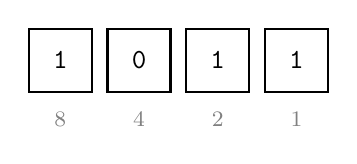
\begin{tikzpicture}
      \bitcell{0}{1}{8}
      \bitcell{1}{0}{4}
      \bitcell{2}{1}{2}
      \bitcell{3}{1}{1}
    \end{tikzpicture}
  \end{figure}
  \vspace{2mm}
  \begin{center}
    $8 + 2 + 1 = 11$
  \end{center}
\end{frame}

\begin{frame}
  With \highlight{$n$} bits we can represent every whole number from \highlight{0} to \highlight{2^n - 1}.\\[4mm]
  \begin{center}
    \graytext{four bits reach \ttab{0000} through \ttab{1111}, that is \ttab{0} to \ttab{15}}
  \end{center}
\end{frame}

\begin{frame}
  To go the other way, we repeatedly divide by two. Each remainder is one bit, read from the last up to the first.\\[3mm]
  \begin{center}
    \renewcommand{\arraystretch}{1.3}
    \begin{tabular}{c@{\hspace{6mm}}c@{\hspace{6mm}}c}
      \graytext{number} & \graytext{halved} & \graytext{remainder} \\ \hline
      \ttab{11} & \ttab{5} & \ttab{1} \\
      \ttab{5}  & \ttab{2} & \ttab{1} \\
      \ttab{2}  & \ttab{1} & \ttab{0} \\
      \ttab{1}  & \ttab{0} & \ttab{1} \\
    \end{tabular}
  \end{center}
  \vspace{2mm}
  \begin{center}
    \graytext{reading the remainders upward gives}\hspace{2mm}\highlight{\ttab{1011}}
  \end{center}
\end{frame}

% ------------------------------------------------------------
% hexadecimal
% ------------------------------------------------------------
\begin{frame}{Hexadecimal}
  \begin{center}
    \Large \highlight{\textbf{hexadecimal}}
  \end{center}
\end{frame}

\begin{frame}
  Long bit patterns are hard to read. \highlight{\textbf{Hexadecimal}} replaces each group of four bits with one symbol.\\[4mm]
  \begin{center}
    \renewcommand{\arraystretch}{1.2}
    \begin{tabular}{cc@{\hspace{10mm}}cc}
      \graytext{bits} & \graytext{hex} & \graytext{bits} & \graytext{hex} \\ \hline
      \ttab{0000} & \ttab{0} & \ttab{1000} & \ttab{8} \\
      \ttab{0001} & \ttab{1} & \ttab{1001} & \ttab{9} \\
      \ttab{0010} & \ttab{2} & \ttab{1010} & \ttab{A} \\
      \ttab{0011} & \ttab{3} & \ttab{1011} & \ttab{B} \\
      \ttab{0100} & \ttab{4} & \ttab{1100} & \ttab{C} \\
      \ttab{0101} & \ttab{5} & \ttab{1101} & \ttab{D} \\
      \ttab{0110} & \ttab{6} & \ttab{1110} & \ttab{E} \\
      \ttab{0111} & \ttab{7} & \ttab{1111} & \ttab{F} \\
    \end{tabular}
  \end{center}
\end{frame}

\begin{frame}
  We split the bits into groups of four and write the symbol for each group.\\[6mm]
  \begin{center}
    \ttab{1011} \; \ttab{0110} \\[2mm]
    \graytext{becomes} \\[2mm]
    \highlight{\ttab{B6}}
  \end{center}
\end{frame}

% ------------------------------------------------------------
% two's complement
% ------------------------------------------------------------
\begin{frame}{Signed Numbers}
  \begin{center}
    \Large \highlight{\textbf{signed numbers}}
  \end{center}
\end{frame}

\begin{frame}
  To store negative numbers, we give the leftmost bit a negative weight. This is \highlight{\textbf{two's complement}}.\\[6mm]
  \begin{figure}
    \centering
    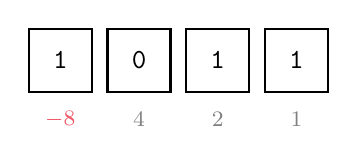
\begin{tikzpicture}
      \node[draw, thick, minimum size=8mm, inner sep=0pt] at (0,0) {\ttab{1}};
      \node[smallgraytext, text=myred] at (0,-0.75) {$-8$};
      \bitcell{1}{0}{4}
      \bitcell{2}{1}{2}
      \bitcell{3}{1}{1}
    \end{tikzpicture}
  \end{figure}
  \vspace{2mm}
  \begin{center}
    $-8 + 2 + 1 = -5$
  \end{center}
\end{frame}

\begin{frame}
  To negate a number we take two steps. Inverting every bit gives the \highlight{\textbf{one's complement}}. Adding one gives the \highlight{\textbf{two's complement}}.\\[5mm]
  \begin{center}
    \renewcommand{\arraystretch}{1.5}
    \begin{tabular}{r@{\hspace{6mm}}l}
      \ttab{0101}          & \graytext{the value \ttab{5}} \\
      \ttab{1010}          & \graytext{one's complement, invert every bit} \\
      \ttab{1011}          & \graytext{two's complement, add one, giving \ttab{-5}} \\
    \end{tabular}
  \end{center}
\end{frame}

\begin{frame}
  This works because a number and its negation add to zero. The carry off the top is discarded.\\[4mm]
  \begin{center}
    \renewcommand{\arraystretch}{1.3}
    \begin{tabular}{r@{\hspace{2mm}}l}
       & \ttab{0101} \\
      $+$ & \ttab{1011} \\ \hline
      \ttab{1} & \ttab{0000} \\
    \end{tabular}
  \end{center}
  \vspace{1mm}
  \begin{center}
    \graytext{so \ttab{1011} really does behave like \ttab{-5}}
  \end{center}
\end{frame}

\begin{frame}
  The same idea explains \ttab{-1}. Adding one to all-ones rolls over to zero, so all-ones must be \ttab{-1}.\\[4mm]
  \begin{center}
    \renewcommand{\arraystretch}{1.3}
    \begin{tabular}{r@{\hspace{2mm}}l}
       & \ttab{1111} \\
      $+$ & \ttab{0001} \\ \hline
      \ttab{1} & \ttab{0000} \\
    \end{tabular}
  \end{center}
\end{frame}

\begin{frame}
  With \highlight{$n$} bits, two's complement covers a balanced range around zero.\\[4mm]
  \begin{center}
    \highlight{-2^{n-1}} \graytext{ to } \highlight{2^{n-1} - 1}
  \end{center}
  \vspace{3mm}
  \begin{center}
    \graytext{four bits run from \ttab{-8} to \ttab{7}}
  \end{center}
\end{frame}

\begin{frame}
  An older scheme, \highlight{\textbf{sign and magnitude}}, uses the top bit only as a sign and the rest as the size.\\[4mm]
  \begin{center}
    \graytext{\ttab{0110} is \ttab{6} \hspace{6mm} \ttab{1110} is \ttab{-6}}
  \end{center}
  \vspace{2mm}
  \begin{center}
    \graytext{it has two zeros and needs more complex arithmetic, so two's complement is preferred}
  \end{center}
\end{frame}

\begin{frame}
  \begin{center}
    Two's complement lets one adder handle both signed and unsigned numbers, which we build next.
  \end{center}
\end{frame}

\end{document}
